\emph{Narratology}, or narrative theory, is a literary science that has experienced considerable development over the last hundred years. The topic of narrative theory has been explored by literary theorists across Europe throughout the twentieth century. Consequently, a number of different typologies and proposals have emerged on how to view the topic of narrative and narrative mode, and how to conduct narrative analysis. \cite{kubicek-vypravec}

In this chapter I introduce some basic narratological concepts. Next, I show a selected typology to demonstrate its relevance to this thesis, ????? and focus on the application of narrative theory to creative writing.

\section{Foundations of Literary Theory and Narratology}


\subsection{Forms of Narrative by Person}

\emph{Person} is a linguistic category of verbs, on the basis of which the primary forms of narrative are distinguished. In addition to verbs, this form is also manifested in personal and possessive pronouns and some special conjunctions.

\paragraph{First-person narrative} is a mode of literary narrative in which the narrator tells the story in first-person singular. Traditionally, first-person narrative reduces the omniscience of the narrator to the subjective perspective, often given by the main character.\cite{vlasin-slovnik}

Nevertheless, there are several modes of first-person narration. These modes differ in the level of subjectivity. \cite{dolezel-narativni-zpusoby}

\paragraph{Third-person narrative} is a mode that is realized in third person singular. Unlike the first-person narrative, the narrator is traditionally in the role of an objective observer. However, in modern literature we can encounter different levels of objectivity. Therefore, the differences between the semantic aspects of first and third person narrative are suppressed. Consequently, the main distinction depends on the syntactic structures of these forms. \cite{vlasin-slovnik}

\paragraph{Other modes of narrative} also exist. There is the \emph{second-person narrative}, which is less frequent narrative mode. We can also encouter narratives given in plural, but these methods are rarely used.

\subsection{System of Narrative Modes}

From a number of narrative typologies I decided to choose the system proposed by Czech linguist and literary theorist Lubomír Doležel. Doležel's system of narrative modes is captured in the tree diagram in the figure \ref{fig:schema-dolezel}.\cite{dolezel-narativni-zpusoby}

\begin{figure}[ht]
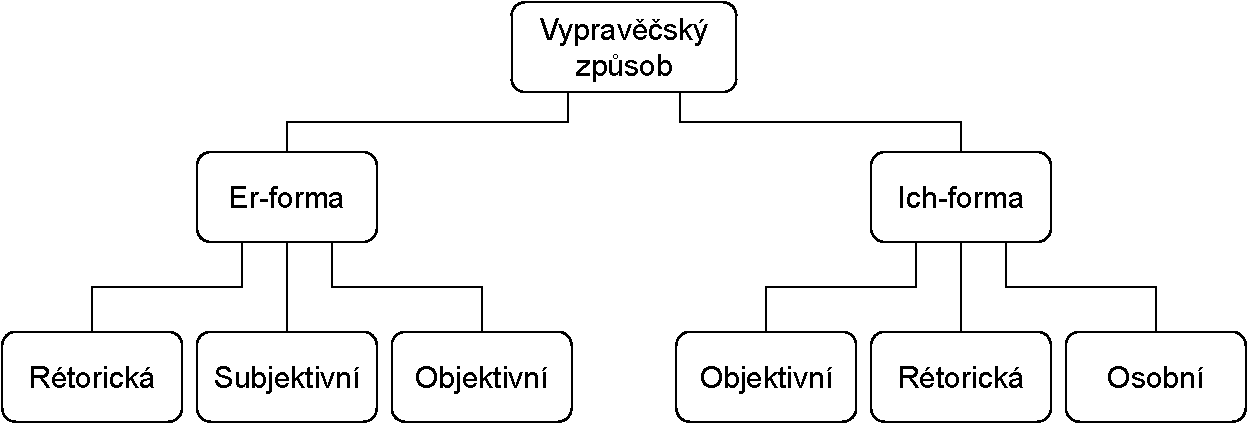
\includegraphics[width=1\textwidth]{data/dolezel-schema.pdf}
\caption{System of narrative modes by Doležel}
\label{fig:schema-dolezel}
\end{figure}



